
\documentclass[11pt]{article}

% My packages
\usepackage{graphicx}
\usepackage[tight,footnotesize]{subfigure}
\usepackage[cmex10]{amsmath}
\usepackage{amsfonts}
\usepackage{amssymb}
\usepackage{textcomp}
\usepackage{bbm}        % Needed for the indicator function
\usepackage{algorithm}
\usepackage{algorithmic}
\usepackage{booktabs}   % Schoener tables!
\usepackage{url}
\usepackage{subfigure}
% \usepackage{robinmath}

% ** This template was prepared for submission to
% ** IEEE Sensors 2012 Conference
% ** using the instructions from
% ** 

% Use english language
\usepackage[english]{babel}

% Bibilography reference in footnotes
\usepackage[style=footnote-dw]{biblatex}
% Package biblatex: '\bibliography' must be given in preamble.
\bibliography{bibliography} % use bib file bibliography.bib

% Implement required margin dimensions
\usepackage[left=2.54cm,right=2.54cm,top=1.25cm,bottom=2.54cm]{geometry}

% Change Title and author fonts to Arial
\usepackage{titlesec}
\usepackage[scaled]{uarial}

\titleformat{\section}{\Large\usefont{T1}{phv}{b}{n}}{\thesection}{1em}{}

\newcommand*{\TitleFont}{%
  \Large\usefont{T1}{phv}{b}{n}%
    \selectfont}

\newcommand*{\AuthorFont}{%
  \normalsize\usefont{T1}{\rmdefault}{m}{n}%
    \selectfont}

% We should really use Times New Roman...
\usepackage{times}


% correct bad hyphenation here, if necessary
\hyphenation{op-tical net-works semi-conduc-tor}


\begin{document}
%
% paper title
% can use linebreaks \\ within to get better formatting as desired
\title{\TitleFont Crowd-sourced citizen-driven mobile sensing of radiation}


% author names and affiliations
% use a multiple column layout for up to two different
% affiliations

\author{
  \AuthorFont Robin Scheibler, Christopher Wang, Kalin Kozhuharov, Joe Moross, Pieter Franken, \\
  \AuthorFont Tomoyuki Furutani, and Keisuke Uehara \\
  \AuthorFont Keio Research Institute at SFC, Fujisawa, Kanagawa, Japan \\
  \AuthorFont \url{robin.scheibler@gmail.com}
}

% no date in the title
\date{}

% make the title area
\maketitle

% remove page number
\thispagestyle{empty}
\pagestyle{empty}

\section*{Summary}
\label{sec:abstract}
% no \IEEEPARstart

Amid the Fukushima triple meltdown disaster of 2011, the lack of independent,
accurate radiation measurement has been a concern. As a response, concerned
citizen have started to take upon themselves this challenging task.

We present the design of an affordable mobile radiation sensor system for
independent citizen monitoring and cartography of radioactive contamination.
Historically radiation measurements has had a high entry barrier for technical,
financial, and political reasons. We show how the tremendous advances in
information technology have been a game changer in this field. Notably, we
leverage the open-source software and hardware paradigm can to dramatically
accelerate the development and deployment time of the system.

Our design methodology allowed to prototype and deploy the system in one
month following the Fukushima disaster. Our sensors have been since driven by
volunteers, covering most of North-East Japan with a fine spatial resolution.

\section*{Motivation}
\label{sec:motivation}

Due to the recent triple meltdown at Fukushima Dai-ichi plant that followed the
Great Tohoku Earthquake and Tsunami, radiation fears dormant since Chernobyl
were suddenly awaken.  During the early time of the crisis, all the radiation
measurements were done by the Ministry of Education, Culture, Sports, Science
and Technology (MEXT) as well as the operator of the plant, Tokyo Electric
Power Company (TEPCO), both having a vested interest in controlling the value
of the measurements published. In addition to that the measurement data was
published in a format unsuitable for machine reading and the data was not
released free of rights, making it difficult to use for academic purposes.

Another drawback of this data set is that it is collected by fixed sensors.
Fixed sensors offer a really good temporal resolution, making it suitable for
early detection of new radioactive pollutant release detection. However, it has
a very poor spatial resolution. Since radioactive plume fall-out is notoriously
spotty because of the airborne travel mode \cite{terada2008development}, a high
spatial resolution is needed in order to precisely assess the contamination at
the level of houses. This is necessary for multiple reasons, including, first
of all, to assess the health hazard and plan evacuation areas accordingly, plan
efficiently decontamination work, identify areas still suitable for farming.
To add to the challenge, during a crisis, the availability of Geiger counters,
not normally mass produced, is not guaranteed. A mobile sensing scheme allows
to efficiently use a reduced number of sensors to cover a large area.

Mobile radiation measurements have been done in the past, notably for
Chernobyl\cite{arvela1990mobile}. However, dramatic advances in localization
and information technology have both increased the performance and lowered the
cost of mobile sensing, making it affordable for communities of concerned
citizen.

Recently, such community-driven mobile sensor networks has emerged as a very
efficient way to cover large areas in detail using much fewer sensors than a
fixed network, at the expense of time resolution \cite{aberer2010opensense}. In
the case of radiation contamination with Cesium 134 and Cesium 137, with
respective half-lives of 2 and 30 years, this is a fair trade-off.

\section*{Results}
\label{sec:results}

Because of the citizen-driven and privately funded nature of the project, the
design needs to be very cost-efficient. Off-the-shelf hardware was used to
create a first system composed of a Geiger counter, a commercial GPS USB
dongle, a micro-controller board and netbook. The audio output of the Geiger
counter was plugged to an Arduino board outputting the count-per-minute (CPM)
every five seconds over serial port. The netbook then aggregates the geographic
location obtained from the GPS and the radiation count and writes it to a file
every five seconds.

The Geiger counter chosen is the Inspector Alert \cite{inspector} that uses an
industry standard \cite{radiological} LND7314 two-inch pancake tube. The Geiger
counter, the Arduino board and the GPS are housed in a waterproof box. This box
is fixed to the side of a car using a simple system of straps that can be
easily fixed on any car by winding up a window on the strap as shown in Fig.
\ref{fig:thefigure} \subref{fig:subfig3}. A long USB cable then links the box
to the netbook inside the car. Suction cups on the back of the box ensure that
the box is firmly attached and do not vibrate, even driving at higher speed on
the highway. Combined to its small form factor, this allows the sensor to be
used in an unobstusive manner on most cars.

The sensor is the workhorse of Safecast\cite{safecast}, a volunteer project
for the mapping of radiation in Japan. The driving of the sensors was crowd
sourced to volunteers based in the contaminated areas in Tohoku. The sensors
unique design allowed it to be used during daily activities, simplifing the
collection of data. As can be observed in \ref{fig:thefigure}
\subref{fig:subfig1}, the spatial resolution allows to finely measure
residential areas.

After collection, the data file produced is manually (as of now) uploaded to an
online database. From this database, comprehensive maps as shown in Fig.
\ref{fig:thefigure} \subref{fig:subfig1} are created and released. Finally, it
is worth noting that the raw data collected is released in the public domain in
machine readable format, allowing it to be easily reused for further research.

\begin{figure}[ht]
\centering
\subfigure[Global map]{
  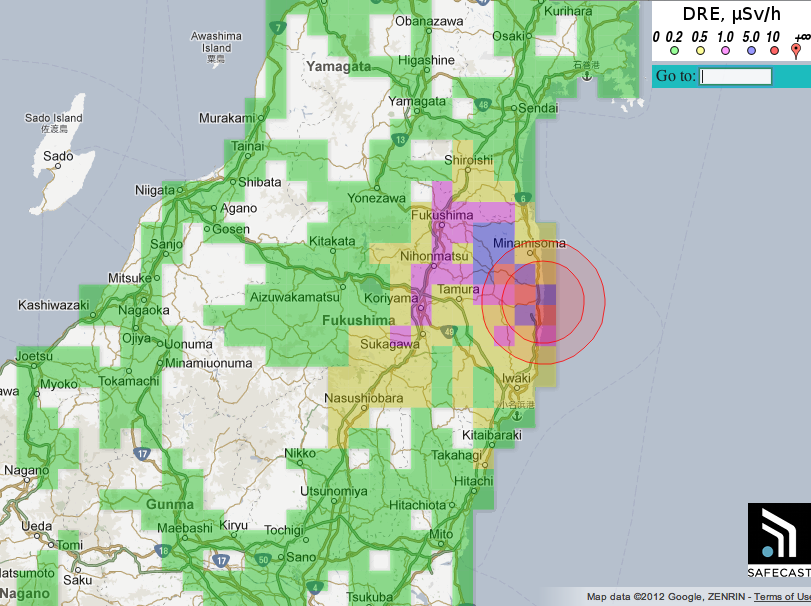
\includegraphics[width=0.3\linewidth]{figures/fusion_map.png}
  \label{fig:subfig1}
}
\subfigure[Individual drive map]{
  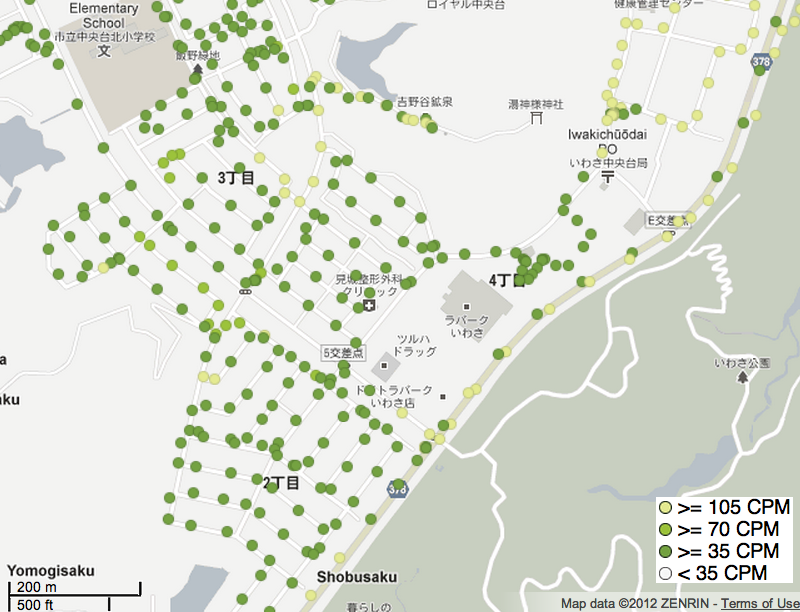
\includegraphics[width=0.3\linewidth]{figures/iwaki_drive.png}
  \label{fig:subfig2}
}
\subfigure[The sensor]{
  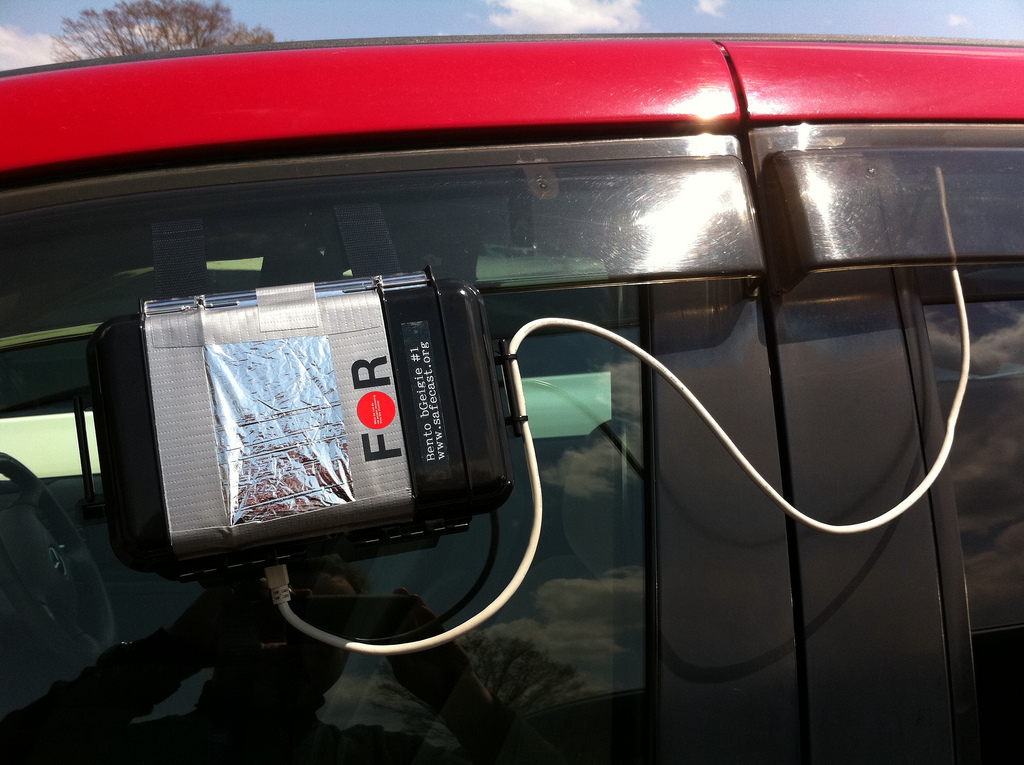
\includegraphics[width=0.3\linewidth]{figures/bgeigie.jpg}
  \label{fig:subfig3}
}
  \caption[The Figure]{ 
            \subref{fig:subfig1} Global map of collected data for the Fukushima
            prefecture.  Each square is color coded according to the average
            dose rate in the area covered.
            \subref{fig:subfig2} Individual drive map. Every point correspond to a
            single measurement. We can observe how it is possible to densely
            cover residential areas.
            \subref{fig:subfig3} The sensor fixed on a car. The box contains the
            Geiger counter a micro-controller to count the pulses from the
            counter, a GPS USB dongle and small USB hub. We can see the USB
            cord that links to the netbook in the car.  
  }
\label{fig:thefigure}
\end{figure}

%\section*{Acknowledgment}
%eio, Tokyo Hackerspace, ...
%The authors would like to thank...
%more thanks here


% trigger a \newpage just before the given reference
% number - used to balance the columns on the last page
% adjust value as needed - may need to be readjusted if
% the document is modified later
%\IEEEtriggeratref{8}
% The "triggered" command can be changed if desired:
%\IEEEtriggercmd{\enlargethispage{-5in}}

% references section

%% this is required to also have a recap. list of references.
% \printbibliography

% We don't use standard bibliography in this paper
% can use a bibliography generated by BibTeX as a .bbl file
% BibTeX documentation can be easily obtained at:
% http://www.ctan.org/tex-archive/biblio/bibtex/contrib/doc/
% The IEEEtran BibTeX style support page is at:
% http://www.michaelshell.org/tex/ieeetran/bibtex/
% \bibliographystyle{IEEEbib}
% argument is your BibTeX string definitions and bibliography database(s)
% \bibliography{IEEEabrv,bibliography}

% that's all folks
\end{document}


